\documentclass[11pt]{article}
\usepackage{graphicx} %for displaying images
\usepackage{float}

%----------------------------------------------------------------------------------------
%	TITLE SECTION
%----------------------------------------------------------------------------------------
\title{	
	\normalfont\normalsize
	\textsc{Old Dominion University}\\ % Your university, school and/or department name(s)
	\vspace{25pt} % Whitespace
	\rule{\linewidth}{0.5pt}\\ % Thin top horizontal rule
	\vspace{20pt} % Whitespace
	{\huge Assignment one}\\ % The assignment title
	\vspace{12pt} % Whitespace
	\rule{\linewidth}{2pt}\\ % Thick bottom horizontal rule
	\vspace{20pt} % Whitespace
}
\author{\LARGE Joshua Gahan} % Your name
\date{\normalsize\today} % Today's date (\today) or a custom date

\begin{document}
	\pagenumbering{gobble}
	\maketitle %render title
	\newpage
	\pagenumbering{arabic}
	
	\section{Curl & Post}
		 \hspace{10mm}In this section we demonstrate knowledge of the curl command by \\ 
		 using it to post data to httpbin.org/post \\
		 \begin{figure}[h!]
		 	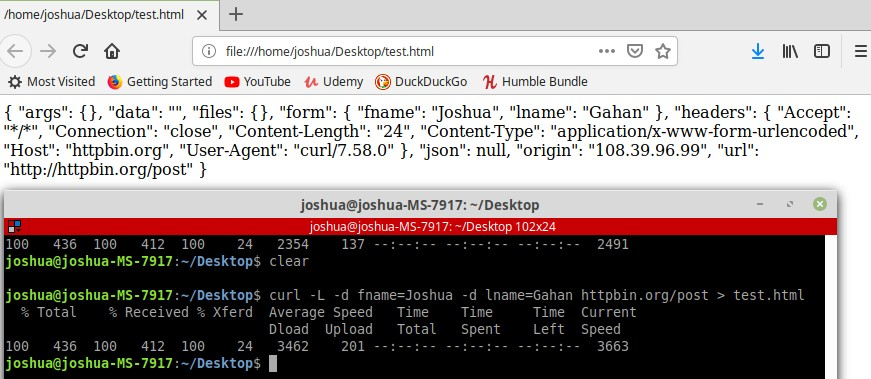
\includegraphics[scale=0.5]{resources/curl.jpg}
		 	\caption{Curl and Post}
		 \end{figure}
		 
	\section{Python Script}
		\hspace{10mm}Here we discuss and demonstrate the usage of python to find and \\ retrieve the byte size of pdf files found in links within a user provided url. \\
		
		\subsection{Retrieval of URIs in Seed URI for parsing }
			\hspace{10mm}For retrieving the URIs within the seed URI we utilize the 
			popular BeautifulSoup library. After retrieving the URIs within \textless a\textgreater\ tags, we
			then apply regex matching to filter out dummy hrefs.  
		\begin{figure}[H]
			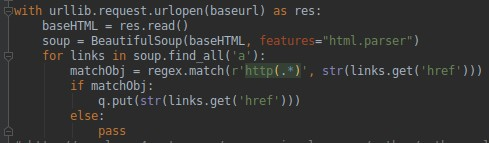
\includegraphics[scale=0.9]{resources/getURLs.jpg}
			\caption{Retrieve URIs}
		\end{figure}
			\hspace{10mm}Links that have passed regex matching are then pushed onto "q," an object of class Queue. This object is used as will be seen below. 
		
		\subsection{Task allocation of found URIs}
			\hspace{10mm}For this project, we have chosen to utilize multithreading. We feel
			that this was the correct decision, as the scraping operation is I/O bound and 
			we can significantly improve the speed of the program with a little extra overhead. In the following, we dynamically create worker threads which pull URIs off the Queue object discussed above. These workers then perform the given "scrapePdfContentLength" function logic. Finally we pause with q.join() and await thread completion. 
			\begin{figure}[H]
				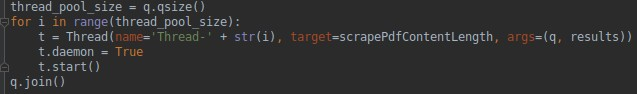
\includegraphics[scale=0.7]{resources/multithread.jpg}
				\caption{Spawning workers}
			\end{figure}
		\subsection{Verify PDF type and retrieve byte size}
			\hspace{10mm}Within each thread, we perform the following function. We first check to 
			ensure that the MIME type is equal to application/pdf and the 'Content-Length' header is
			present.  If this is the case, a formatted string is pushed onto the results list for output within the main program. It is important to note here that python's list datatype is threadsafe. 
			\begin{figure}[H]
				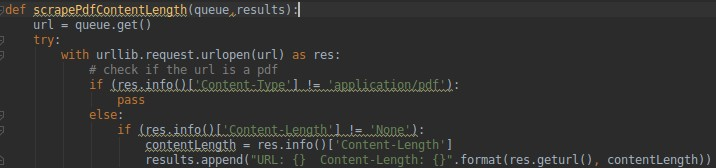
\includegraphics[scale=0.6]{resources/pdfCheck.jpg}
				\caption{Parse and verify candidate links}
			\end{figure}
		\subsection{Demonstration of working program}
		\subsubsection{http://www.cs.odu.edu/~mln/teaching/cs532-s17/test/pdfs.html}
		\begin{figure}[H]
			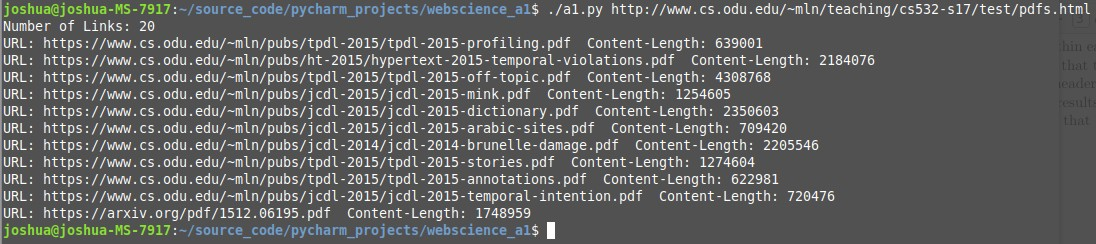
\includegraphics[scale=0.4]{resources/mln.jpg}
			\caption{Running Script on required URL}
		\end{figure}
		
		\newpage 
		\subsubsection{https://en.wikipedia.org/wiki/Python\textunderscore(programming\textunderscore language)}
		Demonstrated on a large seed URL filled with many broken links
		\begin{figure}[H]
			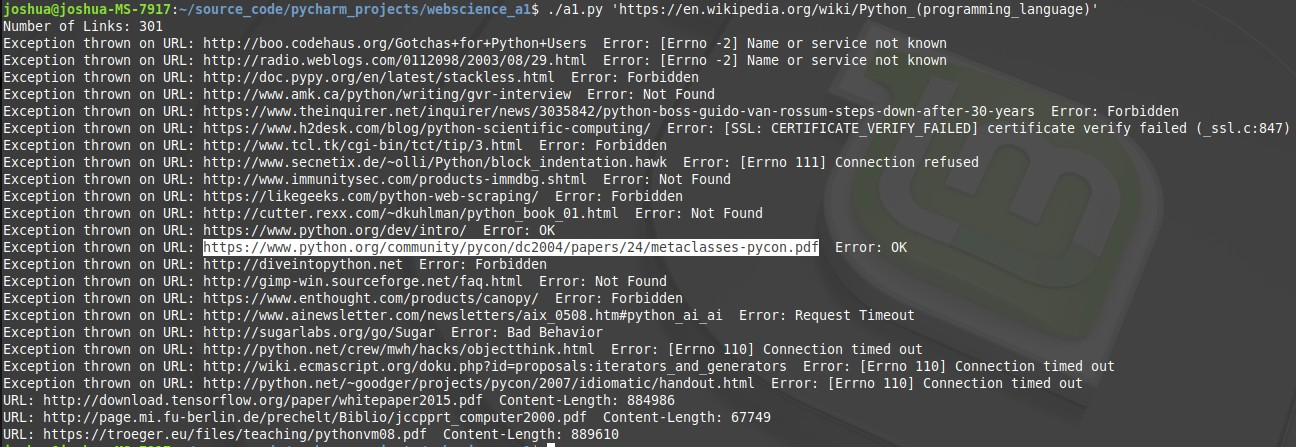
\includegraphics[scale=0.4]{resources/python.jpg}
			\caption{Running Script on Python Wikipedia page}
		\end{figure}
		\subsubsection{https://www.yahoo.com}
		Finally, a run of the script on a url that you would not expect to find any pdfs on. 
		\begin{figure}[H]
			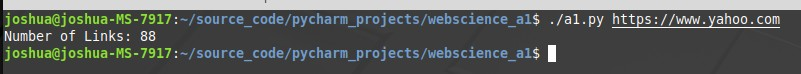
\includegraphics[scale=0.4]{resources/yahoo.jpg}
			\caption{Running Script on yahoo.com}
		\end{figure}
		
	
			
		
	\section{bow-tie graph}
		\hspace{10mm}Here we analyze an edge graph of a theoretical network and identify nodes that belong
		to the following categories: IN, SCC, OUT, TENDRILS, TUBES, and Disconnected. Nodes were categorized by the criteria found at https://www.harding.edu/fmccown/classes/archive/comp475-s13/web-structure-homework.pdf . Where appropriate, phrasing has been borrowed from these definitions.    
		\begin{figure}[H]
			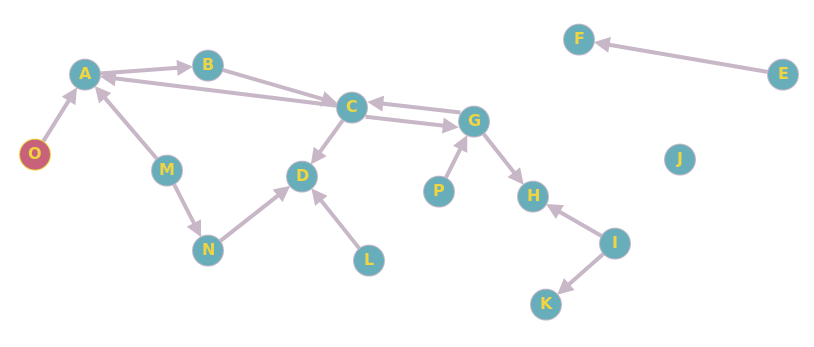
\includegraphics[scale=0.5]{resources/graph.png}
			\caption{Theoretical Graph, graph built with http://graphonline.ru/en/}
		\end{figure}
		\subsection{IN}
		Our IN nodes are O, P, I, and M. These nodes have out-links to SCC, Tendrils or tubes, but have no
		in-links from IN pages. 
		\subsection{SCC}
		Our SCC nodes are A, B, C, and G.  Each of these nodes can access the others through some path, and all have in-links either from INs or other SCCs.
		\subsection{OUT}
		Our OUT nodes are H, K, and D. Each of these nodes can be accessed by in-links but have no out-links to other nodes. 
		\subsection{Tendrils}
		Our Tendril is N . This node can only be reached from M, and it only has an out-link to D (and OUT)
		\subsection{Tubes}
		N also qualifies as a tube. it has in-links from from M (IN) and an out-link to D (OUT). It is not
		connected to any SCC. 
		\subsection{Disconnected}
		Our disconnected nodes are J, E, and F.  These nodes are note part of the network (despite the 
		in-link from E to F)
		
		
	
	
\end{document}